\documentclass{article}
\usepackage{amsmath, amsfonts, amsthm, amssymb}  

\usepackage{secdot}
\usepackage{epsfig}
\usepackage{cprotect}
\usepackage[T1]{fontenc}
\usepackage{epstopdf}
\usepackage{url}
\usepackage{hyperref}
\usepackage{rotating}
\usepackage{graphicx}
\usepackage{caption}
\usepackage{subcaption}
\usepackage{multirow}
\usepackage{amsmath}
\usepackage{setspace}
\usepackage{array}
\usepackage{fancyhdr}
\usepackage{lastpage}
\usepackage[T1]{fontenc}

\usepackage{geometry}
\geometry{letterpaper, left=1in, right=1in, top=1in, bottom=1in}

\pagestyle{fancy}
\fancyhf{}
\rhead{\thepage/\pageref{LastPage}}
\lhead{OSU ECEN 3233 - Logic Design - Fall 2021}
\rfoot{\LaTeX}


% ----- Identifying Information -----------------------------------------------
\newcommand{\myassignment}{Lab 2: Hardware-based Simplified Data Encryption Standard (S-DES)}
\newcommand{\myduedate}{Assigned: Tuesday 9/28; Due \textbf{Monday 10/15} (midnight)}
\newcommand{\myinstructor}{Instructor: James E. Stine, Jr.}
% -----------------------------------------------------------------------------

\begin{document}
\begin{center}
  {\huge \myassignment} \\
  {\large \myduedate} \\
  \begin{flushright}
  \myinstructor \\
  \end{flushright}
\end{center}

\section{Introduction}

Digital systems are important in all areas of society and using
combinational logic is a key element to this
development~\cite{10.5555/2815529}.  This
laboratory will give you more experience with combinational logic
for digital logic.  
Security is becoming a major item for all devices.  It also essential
to devices we use every day, such as cellular phones and computers.
This laboratory will deal with a security cipher that was important in
the 1990s.  However, this security encryption standard, called Data
Encryption Standard (DES)~\cite{fips463}, fell out of favor because we could use
digital logic to help break into these devices.

For this laboratory, we are going to develop a version of DES in two
parts.  The first part will involve designing the
DES encryption and decryption units found in this laboratory,
and second laboratory which we will
use for our project will be a cracker or a
device that can break into the device via hardware.
Security is not only important but many people feel that its one of the most important
topics that engineers
need to learn in the 21st century.  Therefore, I
believe this laboratory will be a great experience in learning some
security and the basics related to making sure someone does not have
unwanted guests within their systems.  The ideas can also be
translated easily into more advanced cryptographic systems, such as
Advanced Encryption Standard (AES) and SHA 256 hash function that is
commonly used in bitcoin.

The DES uses a symmetric-key algorithm for the encryption of data.
Symmetric cryptography just means that the keys can be used both for
encryption and decryption.  Although symmetric-key algorithms can use
the keys both ways, they sometimes are different using some simple
transformations between the two.
% Add stuff on ciphertext and plaintext
The original DES uses a $56$-bit key and a $64$-bit block size.  It
also computes the cipher or translated message in $16$
rounds. Although we could easily create this logic within our Field
Programmable Gate Array (FPGA), it would take a significant amount of
work to ``crack'' or break the message given the time we have in this
class. So, we will use something called a Simplified DES (S-DES)
algorithm which is almost identical to DES albeit smaller in
size~\cite{SchaeferEdwardF1996ASDE}.
The S-DES encryption algorithm takes an $8$-bit block of plaintext
(e.g., \verb!1011_1101!) and a $10$-bit key as input and
produces an $8$-bit block of ciphertext as output.
Similarly, the S-DES decryption algorithm takes an
$8$-bit block of ciphertext and the \textbf{same}
$10$-bit key used to produce that
ciphertext as input and produces the original $8$-bit block of
plaintext.

The S-DES encryption algorithm involves five functions: an initial
permutation (IP); a complex function labeled f\textsubscript{K}, which involves both
permutation and substitution operations and depends on
a key input; a simple permutation function that switches (SW) the two
halves of the data; the function f\textsubscript{K} again; and finally
a permutation
function that is the inverse of the initial permutation
(IP\textsuperscript{-1}).
Although this sounds complicated, it is just simple blocks where the
inputs are used to produce outputs (all in bits).  

\subsection{Security Basics}

Encryption security can be broken down into the basic idea of using a password
or a key to grant access to information.  The message that we want to encrypt is
known as the \textit{plaintext} and the resulting encrypted message is known as the
\textit{ciphertext}.  DES is what is referred to as a symmetric-key algorithm, where the
same key is used to encrypt and decrypt information.  Symmetric-key algorithms
also benefit from straightforward decryption operations: decryption is either
the exact same as encryption or all the steps from encryption simply performed
in reverse-order.  DES fits into the latter category.  The block diagram of
cryptographic hardware operations is shown in Figure~\ref{crypto_hw.png}.
\begin{figure}
  \centering
  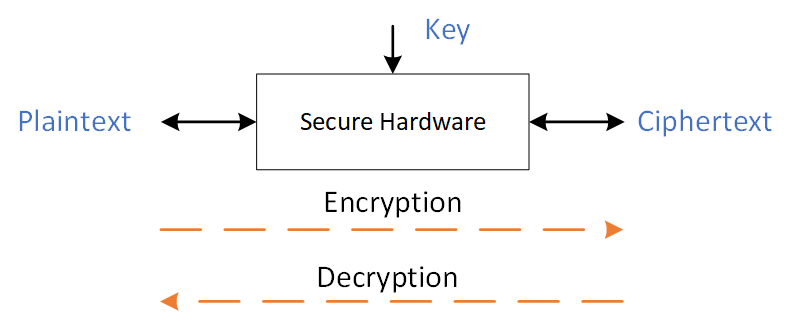
\includegraphics[scale=1.50]{crypto_hw.png}
  \caption{Basic Symmetric Cryptographic Hardware Block Diagram}
  \label{crypto_hw.png}
\end{figure}

\subsection{Rotation}

One of the most common operations in cryptography is called rotation.
Rotation is similar to shifting except anything that is shifted out of
a block gets put back into the block on the other side.  In other
words, a rotation or sometimes called a circular shift is an operation
similar to shift except that the bits that fall off at one end are put
back to the other end.  It is easy to see this as an example.

If we have $n$ that is stored using $8$ bits.
A left rotation of \verb!n = 1110_0101! by $3$ makes
\verb!n = 0010_1111! (Left shifted by 3 and first 3 bits are put back
in least-significant positions.  Fortunately, SystemVerilog (SV) makes
rotation and shifting easy to create with bit-swizzling.

Bit swizzling is SV is achieved with the curly braces \{ and \}.
Using an example from our textbook~\cite{10.5555/2815529}, where $y$ is
given as a $9$-bit value
$c_2c_1d_0d_0d_0c_0101$ using bit swizzling operations.  This can be
created in SV by the following statement.
\begin{verbatim}
assign y = {c[2:1], {3{d[0]}}, c[0], 3’b101};
\end{verbatim}
In reality, the The \{\} operator is used to concatenate busses. The
\verb!{3{d[0]}}! indicates three copies of \verb!d[0]!.
As stated in our textbook do not confuse the $3$-bit binary constant
\verb!3‘b101! with a bus named $b$.
It is important to note that it is critical to specify the length of
$3$ bits in the constant; otherwise, it would have had an unknown
number of leading zeros that might appear in the middle of $y$.
If $y$ were wider than $9$ bits, zeros would be placed in the most
significant bits.

\section{Simplified DES}

Simplified DES uses lots of rotations, swapping or sometimes called
switching, and the use of the exclusive OR operation. The exclusive OR
or xor is useful in that it can be utilized for numbers that have
properties that are sometimes called modular arithmetic.  We will not
go into the theory behind this idea, but you are welcome to explore
more of cryptography in this great text~\cite{10.5555/1721909}.

The symmetric-based cryptographic
algorithm of Simplified or S-DES block diagram
can be seen in
Figure~\ref{SDES_block.png}.  Although Figure~\ref{SDES_block.png}
looks intimidating, it is just simple combinational logic for each
block.  This will be excellent practice in trying to create some
combinational logic from scratch as well as honing some excellent
debugging skills.  
\begin{figure}
  \centering
  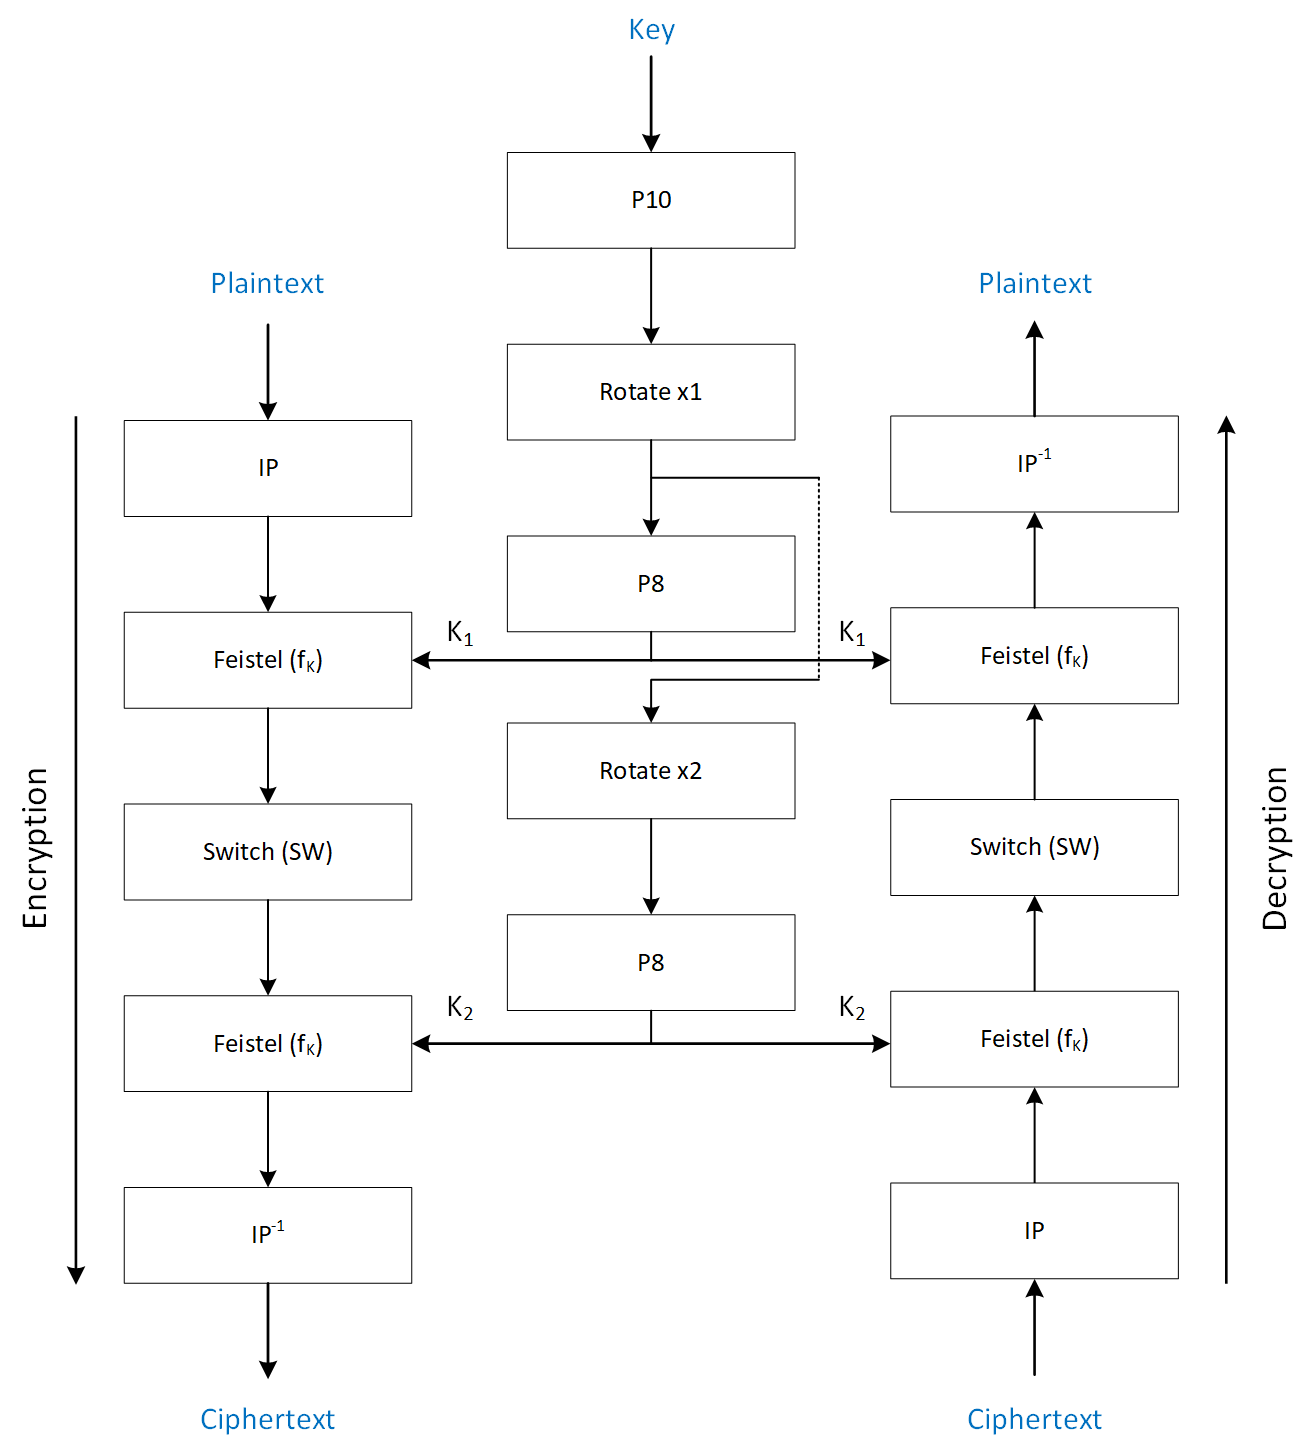
\includegraphics[scale=0.95]{SDES_block.png}
  \caption{S-DES Block Diagram}
  \label{SDES_block.png}
\end{figure}
In order to break down each block, we will break this into two
sections : one for key generation (i.e., $K_1$ and $K_2$) and the
other for the basic symmetric cryptographic algorithm.

\subsection{Key Generation}

In order to start, the best place to start is producing the key
generation.  The key generation involves three basic blocks:
\begin{enumerate}
\item P10 : $10$-bit permutation
\item Rotation
\item P8 : $8$-bit permutation
\end{enumerate}
Each block produces two keys: $K_1$ and $K_2$ that get used during
encryption and decryption.  More advanced algorithms, for example for
those found in~\cite{10.5555/1721909}, use the same option but
typically have more keys to produce more security.

To understand the
permuations, let's start with a vector called \verb!A[9:0]!.  Therefore, P10 is the following:
\begin{verbatim}
{A[7], A[5], A[8], A[3], A[6], A[0], A[9], A[1], A[2], A[4]}
\end{verbatim}
And, P8 is the following:
\begin{verbatim}
{A[4], A[7], A[3], A[6], A[2], A[5], A[0], A[1]}
\end{verbatim}
It is important to note that P8 actually does not use all of the
$10$-bit vector but only utilizes part of the vector to produce an
$8$-bit output.
Again, it is not important to understand why these permutations are
done this way, but just that you need to follow the procedure
correctly.  Later on, we will discuss how to verify each section is
working correctly.

Rotation is performed as explained earlier except that the first block is
rotated once and the second block rotates twice.  The only caveat here
is that \textbf{each rotation} should be done by separating each
$10$-bit block
into $5$-bits or broken into two groups.  Let's try an example to
illustrate this by showing a rotation by two ($2$) on \verb!10_1011_1000!.
To accomplish this rotation, first break the $10$-bits into two groups
of $5$-bits or \verb!1_0101! and \verb!1_1000!.   Then, the rotation
is done on each block separately or:  \verb!1_0110! and \verb!0_0011!
That is, the final rotation will be the concatenation of these two
items or \verb!10_1100_0011!.

\subsection{S-DES encryption or decryption}

As stated earlier, S-DES is a symmetric cryptographic algorithm in
that it can be done either way for encryption or decryption.  It is
important to understand the order as shown in
Figure~\ref{SDES_block.png} making the correct direction is utilized
for encryption or decryption.  Again, this block is another group of simple
combinational logic blocks with it broken down into four basic
blocks:
\begin{enumerate}
\item Initial Permutation (IP)
\item Feistel Block ($f_K$)
\item Switch or Swapping (SW)
\item Inverse Permutation (IP\textsuperscript{-1})
\end{enumerate}

Assuming that the input to this sequence is \verb!PT[7:0]!
The Initial Permutation (IP) block is easily created by:
\begin{verbatim}
IP = {PT[6], PT[2], PT[5], PT[7], PT[4], PT[0], PT[3], PT[1]}
\end{verbatim}
Swapping is just swapping each $8$-bit blocks by $4$-bits.  For
example, if the input is \verb!FB[7:0]! the swap would be
\begin{verbatim}
SW = {FB[3:0], FB[7:4]}
\end{verbatim}
Finally, the inverse permutation or IP\textsuperscript{-1} is created
similarly to the IP block:
\begin{verbatim}
IP^{-1} = {SW[4], SW[7], SW[5], SW[3], SW[1], SW[6], SW[0], SW[2]}
\end{verbatim}

\subsubsection{Feistel Block}

The main part of this section is called the Feistel block that is
named after the German-American cryptographer Horst Feistel.  Horst
Feistel main work was in developing ciphers for IBM and we call this
block the Feistel block after his pioneering work.

The Feistel block or $f_K$ basically performs the exclusive OR'ing or
XORing on blocks of $8$-bits.  Inside this Feistel block are key elements of
symmetric cryptographic algorithms called substitution boxes or
sometimes abbreviated as S-box.  S-boxes are utilized in block ciphers to
to obscure the relationship between the key and the ciphertext, thus
ensuring Shannon's property of confusion~\cite{10.5555/1721909}.   For
this lab, I will provide the S-boxes for you so you just have to
compute the Feistel block correctly.  The order of operations in the
Feistel block are as follows:
\begin{enumerate}
\item Split the $8$-bit IP output into two separate blocks of $4$-bits:
  \verb!F[3:0]! and \verb!S[3:0]!.
\item Create the expansion/permutation (EP) operation by replicating
  the second block only as:
  \begin{verbatim}
    EP[7:0] = {S[0], S[3], S[2], S[1], S[2], S[1], S[0], S[3]}
\end{verbatim}
\item XOR the EP block with the key ($K_i$)
\item Take the output of the XOR block and go into two S-boxes where
  the first S-box uses \verb!XOR_out[7:4]! and the second S-box uses
  \verb!XOR_out[3:0]! producing \verb!S0[1:0]! and \verb!S1[1:0]!, respectively.
\item The next block in the Feistel block is called the P4 block or
  $4$-bit permutation and
  it takes the output of the S-boxes and groups it into $4$-bits :
  \verb!P4_in[3:0] = S0[1:0], S1[1:0]!  and produces the output
\begin{verbatim}
P4_out[3:0] = {P4_in[2], P4_in[0], P4_in[1], P4_in[3]}
\end{verbatim}
  \item Finally, the P4 output is XORed with \verb!F[3:0]! as
    \verb!xor_out = P4_out[3:0] xor F[3:0]! and output as
    \verb!xor_out!, \verb!S[3:0]!.
\end{enumerate}
\begin{figure} [t!]
  \centering
  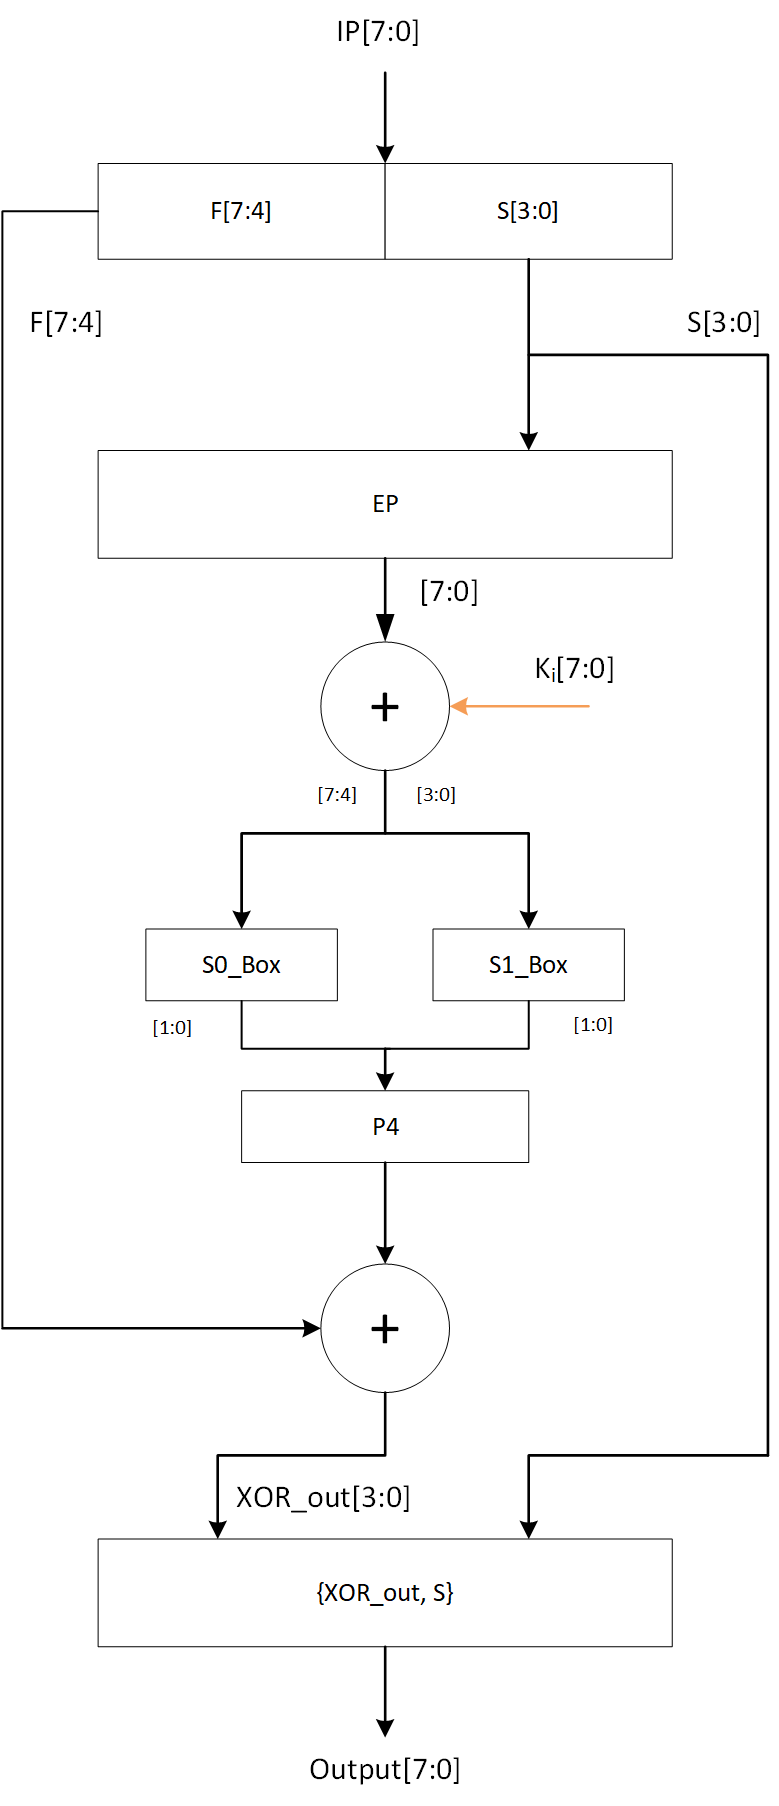
\includegraphics[scale=0.6]{feistel.png}
  \caption{Feistel ($f_K$) Block}
  \label{feistel.png}
\end{figure}

Figure~\ref{feistel.png} shows the basic block diagram of what the
Feistel algorithm is doing.  
Again, this does look like a lot of work but it is quite
straightforward.
Also, the Feistel block operates with two keys.
Therefore, pay attention to Figure~\ref{SDES_block.png} for each key
$K_1$ and $K_2$ and its use for either encryption or decryption.
Please also note in Figure~\ref{SDES_block.png} does two Feistel
computations, so you will have to use this block twice per operation
(e.g., encryption).

\subsection{Encryption or Decryption}

Encryption or decryption can be produced from the same block as shown in
Figure~\ref{SDES_block.png}.  This is where the name symmetrical
cryptographical algorithm comes from.  The only difference is the
order of operations and what Key is being
used (i.e., $K_1$ or $K_2$).  Your top diagram should have an input
that tells it whether to
encrypt or decrypt your block.
  
\section{Tasks}

Most of the blocks and their operation
have been given to you to help you understand the
problem better.
For those that are interested in more about cryptography and how
hardware can impact the future, I encourage you to read more about it
through searching on the Internet as well as this great
reference~\cite{10.5555/1721909}.
One of the hard parts of any engineering problem is
to understand what is going on and making sure you are correct.
Therefore, digital designers rely heavily on getting good data to make
sure they are right.  Typically, this is done either on paper and
pencil or through software.

We will use software for this approach
and use a piece of software written by Professor Rob Beezer at the
University of Puget Sound in Washington State.  He has graciously
allowed us to use this software for the project and it is great
because it allows you to put vectors in and test them at each stage.
I have slightly modified the User Interface (UI) shown in
Figure~\ref{java_sw.png} to have names that
match the block diagrams on Figure~\ref{SDES_block.png}.  If you need
to install Java on your machine at home or laptop, go to
\url{https://www.oracle.com/java/technologies/downloads/#java16} and
download the appropriate version.
\begin{figure} [t!]
  \centering
  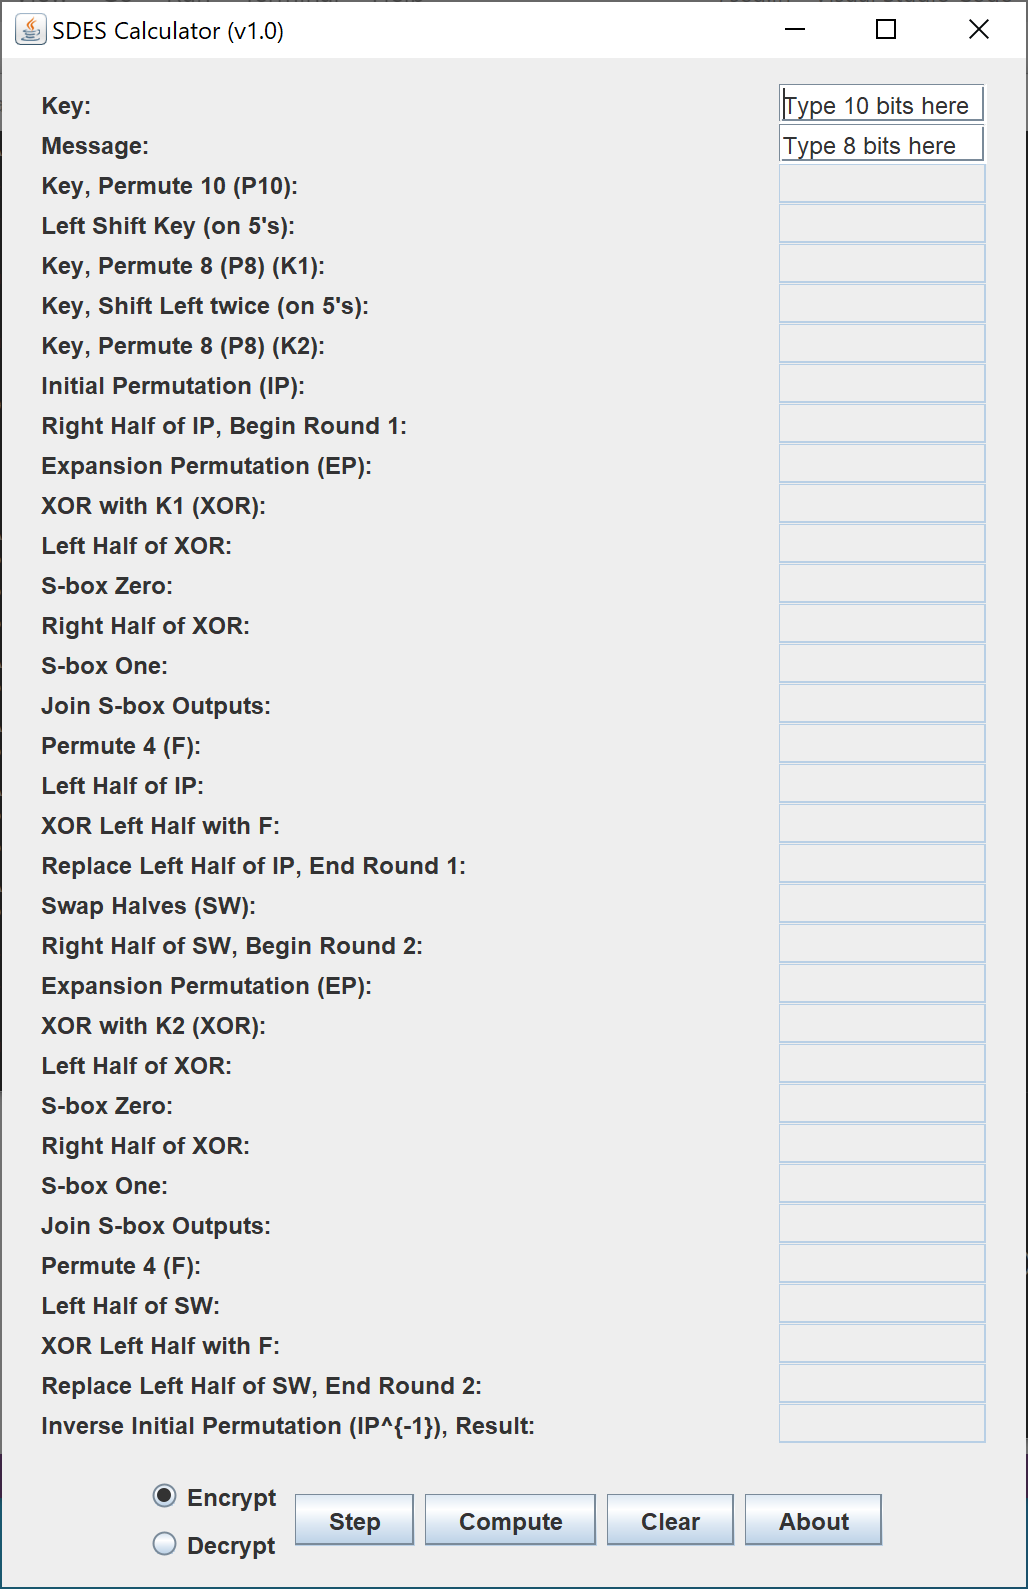
\includegraphics[scale=0.4]{java_sw.png}
  \caption{Java Verification Tool Written by Professor Rob Beezer}
  \label{java_sw.png}
\end{figure}

Verification is hard because there are so many moving parts.  Use the
Java program to verify each block out of the HDL.  Although the Java
works based on bytecodes that are interpreted, I have found that some
machines have problems reading the Java bytecodes.  I am still not
quite sure why this is the case, however, there is an easy fix.
Therefore, I included a
Makefile that I wrote that allows you to compile the Java correctly.
Please type the following if you are having problems running the
code.  To run the tool, type \verb!java SDES! at the command prompt.
\begin{verbatim}
make clean
make
\end{verbatim}
If you cannot run \verb!make! on your Windows box, just type the
\verb!javac! commands found within the Makefile on each Java file.  

The main tasks for this laboratory
will be the following elements:
\begin{enumerate}
  \item Design the S-DES combinatianal block for both encryption and
    decryption in SystemVerilog and simulate with ModelSim.
  \item Use the Java verification tool to help you with verifying the
    correct operation within ModelSim.
  \item Test at least $10$ random messages (i.e., plaintext) using
    $2$ random keys for both encryption and decryption.
  \item After verifying your design with a testbench in ModelSim,
    implement your design on the DSDB board and use the    
    $7$-segment display to display your plaintext and ciphertext.
  \item Use the push buttons, switches, and LEDs to help you input
    your plaintext as well as debug operation and prove that your
    design works on your DSDB board.
\end{enumerate}
Again, there are many parts to this design and based on experience, I
believe it will be easier to debug the key generation first and then
once this works, debug the encryption/decryption next.  The key
generation is slightly easier than operations like the Feistel block,
so it will optimize your design process if you focus on this block
first.  However, I would use the strategy that works the best for you.

\subsection{Testing and Stubbing Code}

You should use the testbenches you utilized for Lab0 and Lab1 to help
you test your design.  The design is completely combinational and
should not be any different in terms of structure than both of these
labs.  To get full credit, you should demonstrate that your design
works for both encryption and decryption by testing at least $10$
plaintext messages using at least $2$ different keys.  This is
basically testing $20$ vectors - the more vectors tested and the
methodology you use could possibly
earn you extra credit on this laboratory.

I have also given you some freebies to help you with this lab.  When
writing HDL or software, it is sometimes useful to \textit{stub} your
code.  A stubbed piece of code is a blank piece of software that has
most of your functions you believe will work for your design.
Fortunately, I have stubbed out your SV for you and you can use this.
Inside the SV, I have also included the \verb!S0_box! and
\verb!S1_box! which are the two substitution boxes you will use for
this laboratory.  Both of the S-boxes work by giving them $4$-bits and
they produce $2$-bits as indicated previously. 

\subsection{Getting to know ModelSim and Debugging}

ModelSim is a professional Hardware Descriptive Language tool for
simulation and verification.  It has many neat features to help you
with debugging.  Although testbenches are the main vehicle for
understanding how to test a digital system, using ModelSim can save
you hours and days in debugging a design.  Therefore, we are also
going to introduce some new features of ModelSim that you should use
to help you with this laboratory. I also encourage you to use the
testbench skills you learned from Lab 1.

The features you will use in ModelSim are the \textit{Sim} and
\textit{Objects} window.  Normally both of these windows are present
when running a DO file, however, sometimes I find that they do not
open properly.  You may need to activate them in the View menu at the
top of ModelSim.  They should look like Figure~\ref{modelsim.png} when
activated.  Both of these windows are utilized with the Wave window.
\begin{figure} [t!]
  \centering
  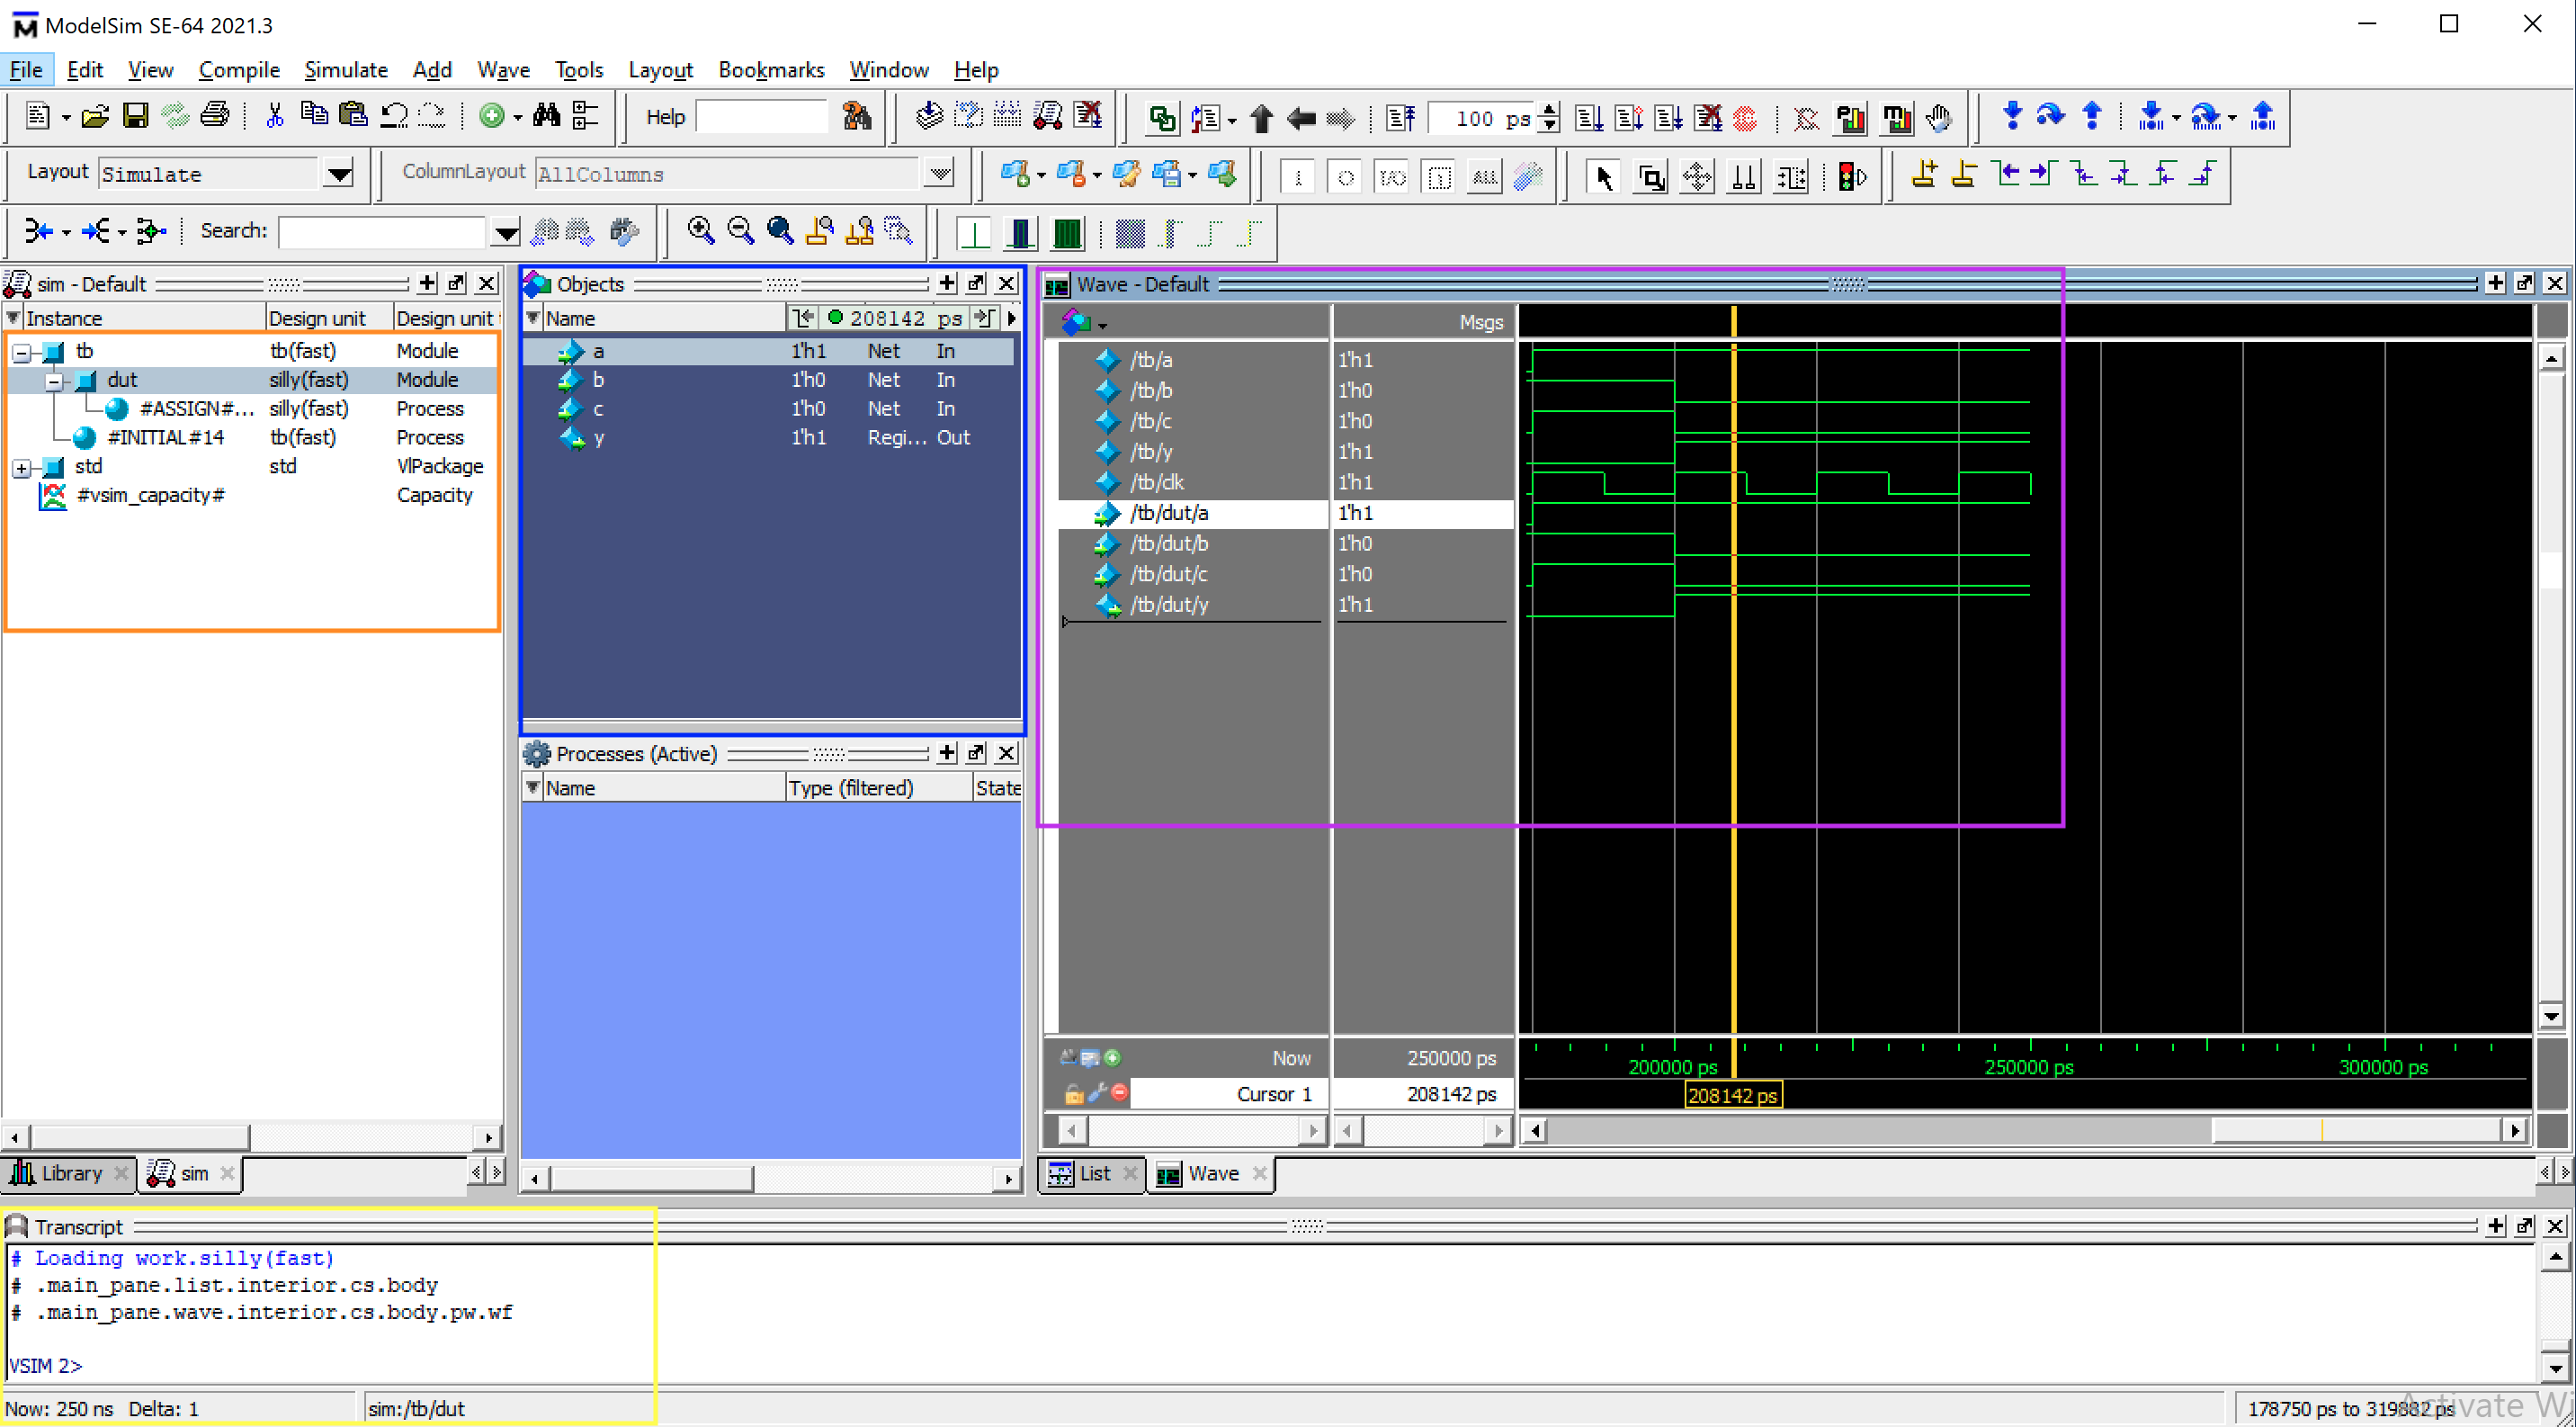
\includegraphics[scale=0.3]{modelsim.png}
  \caption{ModelSim Sim and Objects Window}
  \label{modelsim.png}
\end{figure}

To use the two windows effectively, you should use the \textit{Wave}
to see the data at a certain time.  First, move your cursor to the
time you wish to investigate something - you should see a yellow line
indicating the time you are observing the data.  Next, you
should navigate to the
hierarchy of the module you wish to verify in the \textit{Sim} window
and the \textit{Objects} window will display all signals and values
that for that instance at a given time.  You might need to play around
with using these two windows together with the \textit{Wave} window,
but once you do you will find that its easy to debug what each block
is producing at a given time.

The "sim" window (orange) contains the hierarchy of the design.  The
top level shows the test bench (tb) with a expandable button to the
left.
By clicking the "+" it opens the hierarchy for all modules
instantiated in tb.  Clicking on the name of the instance changes
which objects (blue) are visible in the "objects" window.  You can
also add an
object to the wave by right clicking on the name of the object in the
"objects" window "Add Wave".  Your testbench and modules may use
different names but the same process applies to add signals to the
wave (purple).

You can save the wave by clicking in the wave window then clicking the
brown colored floppy disk icon in the toolbar.  (Third icon from the
left)  The saved file only contains the configuration of the wave not
the actual data. This allows you to recall the wave if you restart
modelsim at a later time.  To recall the wave you can type "do <name
of wave file> in the transcript (yellow).  You can also add this to
the do file so it always pulls up your wave every time the simulation
is run.

Modelsim has many extra features which can greatly aid in your debugging.
First let's discuss some tips and tricks.
\begin{itemize}
\item  If the toolbar gets disorderly, right click in the toolbar and
  select reset.
\item Signals in the wave by default show the full path name.  This can
  be changed to just the lowest level of hierarchy by clicking the
  ``toggle leafs name'' button in the lower left of the wave shown in
  Figure~\ref{modelsim-tips1.png}  
\item Zoom buttons are confusing.  The ``+'' zoom in is mostly useless.
  Use the yellow upside down ``T'' with magnifying glass to zoom in
  at the cursor, as shown in Figure~\ref{modelsim-tips2.png} in red.
\item The ``-'' zoom button works as expected.
\item If you select a signal in the wave viewer, ``Tab'' and ``Shift + Tab''
  will move the cursor to the next transition.
\item A multibit bus can be search for a specific value using the ``Search''
  buttons in the toolbar.  The blue left and right allows to the right of
  the ``Search'' button will search backwards (left) or forwards (right)
  in time, as shown in Figure~\ref{modelsim-tips2.png} in green.
\end{itemize}

At the risk of complicating things the ``data flow'' window can be very
helpful when debuging red X's.  Either in the objects window or the wave
window right click a signal and select ``Add to dataflow''. This opens
a new window where you can right click and select ``ChaseX'' or ``TraceX''.
These allow you to quickly find the source of an X.  If this does not make
sense you can skip.
\begin{figure} [t!]
  \centering
  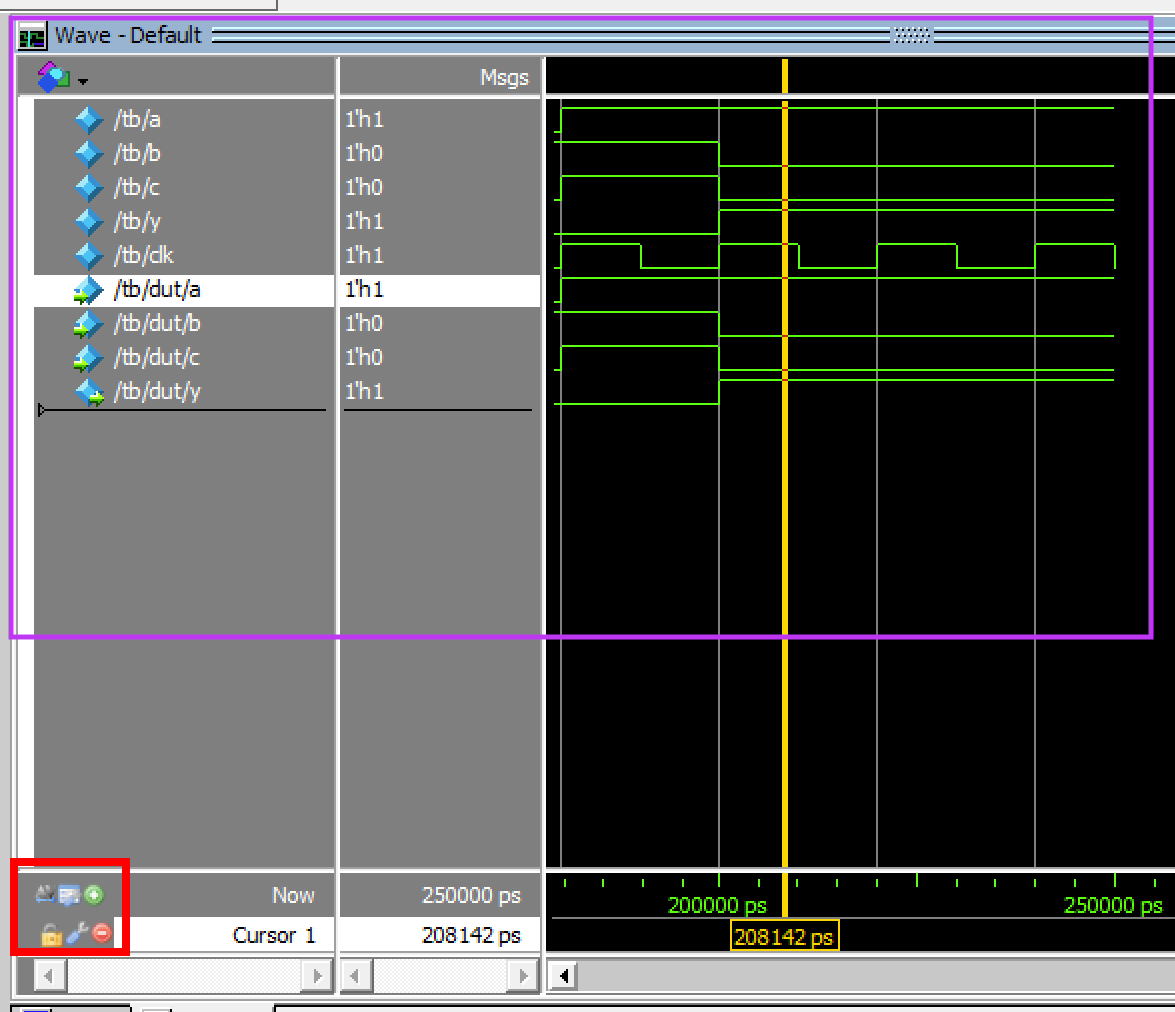
\includegraphics[scale=0.3]{modelsim-tips1.png}
  \caption{ModelSim toggle leafs. In the red box, the left-most box is the ``Now'' row.}
  \label{modelsim-tips1.png}
\end{figure}
\begin{figure} [t!]
  \centering
  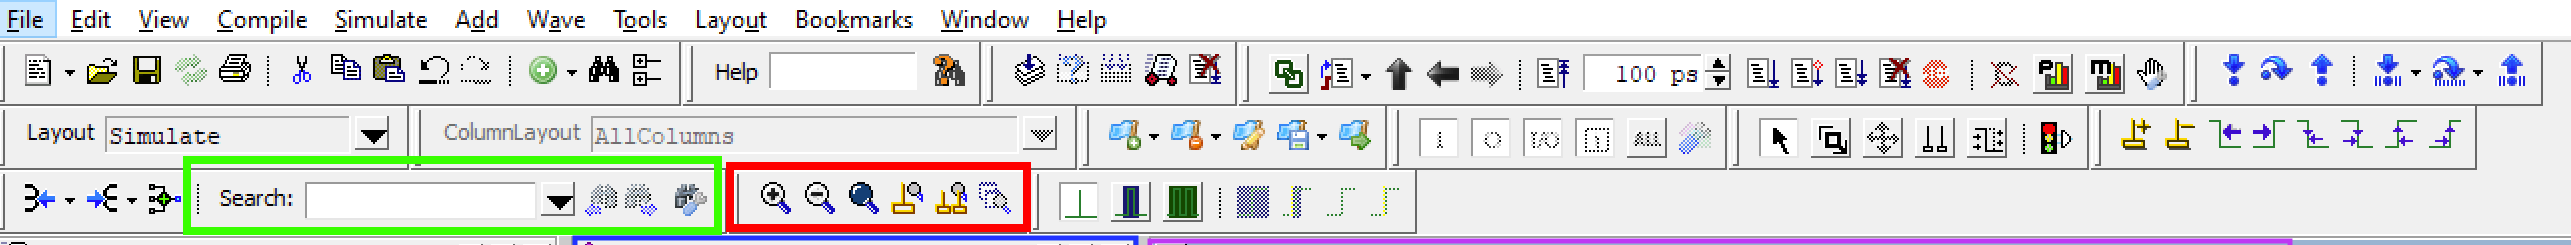
\includegraphics[scale=0.3]{modelsim-tips2.png}
  \caption{Search inside the green box and zoom controls in the red box.}
  \label{modelsim-tips2.png}
\end{figure}

\subsection{Extra Credit}

If you get done early, you can attempt some extra credit.  However, I
would only try this option if you get everything verified within your
design.  One possible option is to adapt the design to perform the
complete DES - this is a big undertaking and only for serious students
who find this topic very interesting and have extra time.

Another possible improvement is to work on optimizing the verification
of your design.  I have included a Java program that I wrote that
outputs multiple values for the S-DES implementation in Java.  You
could use these vectors to self-verify your implementation as in Lab 1.

Yet another piece of extra credit is analyzing how fast you can run
DES through.  This will involve using Vivado to analyze how fast your
design can be and doing some calculations on how fast you can encrypt
and decrypt your data.  

\section{Submission}

You should electronically hand in your HDL (all files that you want
us to see) into Canvas.
You should also take a printout of your waveform 
from your ModelSim simulation.  
Only one of your team members should upload
the files and/or lab report. Please contact
James Stine
(james.stine@okstate.edu) 
for more help.  Your
code should be
readable and well-documented. In addition, please turn in additional
test cases or any other added item that you used. 
Please also remember to document everything in your Lab Report using
the information found in the Grading Rubric.


    
\bibliographystyle{IEEEbib}
\bibliography{lab2}

\end{document}
